\begin{figure}
	\centering
	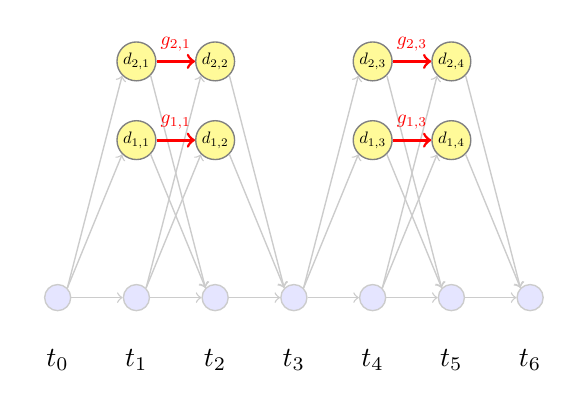
\begin{tikzpicture} 
		\node[circle, fill=blue!10, line width=0.5pt, draw=black!20, minimum size=0.1in](one) at (0,0){};
		\node[circle, fill=blue!10, line width=0.5pt, draw=black!20, minimum size=0.1in](two) at (1,0){}; 
		\node[circle, fill=blue!10, line width=0.5pt, draw=black!20, minimum size=0.1in](three) at (2,0){};
		\node[circle, fill=blue!10, line width=0.5pt, draw=black!20, minimum size=0.1in](four) at (3,0){};
		\node[circle, fill=blue!10, line width=0.5pt, draw=black!20, minimum size=0.1in](five) at (4,0){};
		\node[circle, fill=blue!10, line width=0.5pt, draw=black!20, minimum size=0.1in](six) at (5,0){};
		\node[circle, fill=blue!10, line width=0.5pt, draw=black!20, minimum size=0.1in](seven) at (6,0){};
		
		\node[circle, fill=yellow!40, line width=0.5pt, draw=black!50, minimum size=0.1in, inner sep=1pt](eight) at (1,2){\scalebox{0.6}{$d_{1,1}$}};
		\node[circle, fill=yellow!40, line width=0.5pt, draw=black!50, minimum size=0.1in, inner sep=1pt](nine) at (2,2){\scalebox{0.6}{$d_{1,2}$}};
		\node[circle, fill=yellow!40, line width=0.5pt, draw=black!50, minimum size=0.1in, inner sep=1pt](ten) at (4,2){\scalebox{0.6}{$d_{1,3}$}};
		\node[circle, fill=yellow!40, line width=0.5pt, draw=black!50, minimum size=0.1in, inner sep=1pt](eleven) at (5,2){\scalebox{0.6}{$d_{1,4}$}};

		\node[circle, fill=yellow!40, line width=0.5pt, draw=black!50, minimum size=0.1in, inner sep=1pt](twelve) at (1,3){\scalebox{0.6}{$d_{2,1}$}};
		\node[circle, fill=yellow!40, line width=0.5pt, draw=black!50, minimum size=0.1in, inner sep=1pt](thirteen) at (2,3){\scalebox{0.6}{$d_{2,2}$}};
		\node[circle, fill=yellow!40, line width=0.5pt, draw=black!50, minimum size=0.1in, inner sep=1pt](fourteen) at (4,3){\scalebox{0.6}{$d_{2,3}$}};
		\node[circle, fill=yellow!40, line width=0.5pt, draw=black!50, minimum size=0.1in, inner sep=1pt](fifteen) at (5,3){\scalebox{0.6}{$d_{2,4}$}};

		\draw [->, line width=0.5pt, color=black!20] (one.east) -- (two.west);
		\draw [->, line width=0.5pt, color=black!20] (two.east) -- (three.west);
		\draw [->, line width=0.5pt, color=black!20] (three.east) -- (four.west);
		\draw [->, line width=0.5pt, color=black!20] (four.east) -- (five.west);
		\draw [->, line width=0.5pt, color=black!20] (five.east) -- (six.west);
		\draw [->, line width=0.5pt, color=black!20] (six.east) -- (seven.west);

		\draw [->, line width=0.5pt, color=black!20] (one.north east) -- (eight.south west);
		\draw [->, line width=0.5pt, color=black!20] (two.north east) -- (nine.south west);
		\draw [->, line width=0.5pt, color=black!20] (four.north east) -- (ten.south west);
		\draw [->, line width=0.5pt, color=black!20] (five.north east) -- (eleven.south west);
		\draw [->, line width=0.5pt, color=black!20] (eight.south east) -- (three.north west);
		\draw [->, line width=0.5pt, color=black!20] (nine.south east) -- (four.north west);
		\draw [->, line width=0.5pt, color=black!20] (ten.south east) -- (six.north west);
		\draw [->, line width=0.5pt, color=black!20] (eleven.south east) -- (seven.north west);

		\draw [->, line width=0.5pt, color=black!20] (one.north east) -- (twelve.south west);
		\draw [->, line width=0.5pt, color=black!20] (two.north east) -- (thirteen.south west);
		\draw [->, line width=0.5pt, color=black!20] (four.north east) -- (fourteen.south west);
		\draw [->, line width=0.5pt, color=black!20] (five.north east) -- (fifteen.south west);
		\draw [->, line width=0.5pt, color=black!20] (twelve.south east) -- (three.north west);
		\draw [->, line width=0.5pt, color=black!20] (thirteen.south east) -- (four.north west);
		\draw [->, line width=0.5pt, color=black!20] (fourteen.south east) -- (six.north west);
		\draw [->, line width=0.5pt, color=black!20] (fifteen.south east) -- (seven.north west);
		\draw [->, line width=1pt, color=red] (twelve.east) -- node[above]{\scalebox{0.7}{$g_{2,1}$}}(thirteen.west);
		\draw [->, line width=1pt, color=red] (fourteen.east) -- node[above]{\scalebox{0.7}{$g_{2,3}$}}(fifteen.west); 
		\draw [->, line width=1pt, color=red] (eight.east) -- node[above]{\scalebox{0.7}{$g_{1,1}$}}(nine.west);
		\draw [->, line width=1pt, color=red] (ten.east) -- node[above]{\scalebox{0.7}{$g_{1,3}$}}(eleven.west); 

		\node[rectangle, minimum width=0.3in, minimum height=1.2in,label=below:$t_0$](time0Box) at (0,1){};
		\node[rectangle, minimum width=0.3in, minimum height=1.2in,label=below:$t_1$](time1Box) at (1,1){};
		\node[rectangle, minimum width=0.3in, minimum height=1.2in,label=below:$t_2$](time2Box) at (2,1){};
		\node[rectangle, minimum width=0.3in, minimum height=1.2in,label=below:$t_3$](time3Box) at (3,1){};
		\node[rectangle, minimum width=0.3in, minimum height=1.2in,label=below:$t_4$](time4Box) at (4,1){};
		\node[rectangle, minimum width=0.3in, minimum height=1.2in,label=below:$t_5$](time5Box) at (5,1){};
		\node[rectangle, minimum width=0.3in, minimum height=1.2in,label=below:$t_6$](time6Box) at (6,1){}; 

	\end{tikzpicture}
	\caption{Depiction of which edges increase SOC for the single rate case}
	\label{fig:dSocDiagram}
\end{figure}


